\documentclass[9pt,twoside,lineno]{pnas-new}
% Use the lineno option to display guide line numbers if required.

\templatetype{pnassupportinginfo}
% \readytosubmit %% Uncomment this line before submitting, so that the instruction page is removed.

\title{Conceptualizing and Measuring Resilience to Hazards as Access to Essential Services}
\author{T M Logan and S D Guikema}
\correspondingauthor{T Logan\\E-mail: tomlogan@umich.edu}

\begin{document}

%% Comment/remove this line before generating final copy for submission
% \instructionspage  

\maketitle

%% Adds the main heading for the SI text. Comment out this line if you do not have any supporting information text.
\SItext

\section*{Mapping the access distribution to a resilience curve}

Figure \ref{figS:cdf_to_res} conceptually demonstrates how the distribution of access is mapped to a resilience curve. The four time-states show the progression through the hazard cycle, from pre-disruption, disruption, recovery, and then transformation with future mitigation. Quantifying access to essential services has advantages throughout the hazard cycle that are discussed later in this section. Fundamentally, it allows us to assess the capacity of the system to maintain and restore desired functionality following a disruption.

\begin{figure}[h]
    \centering
    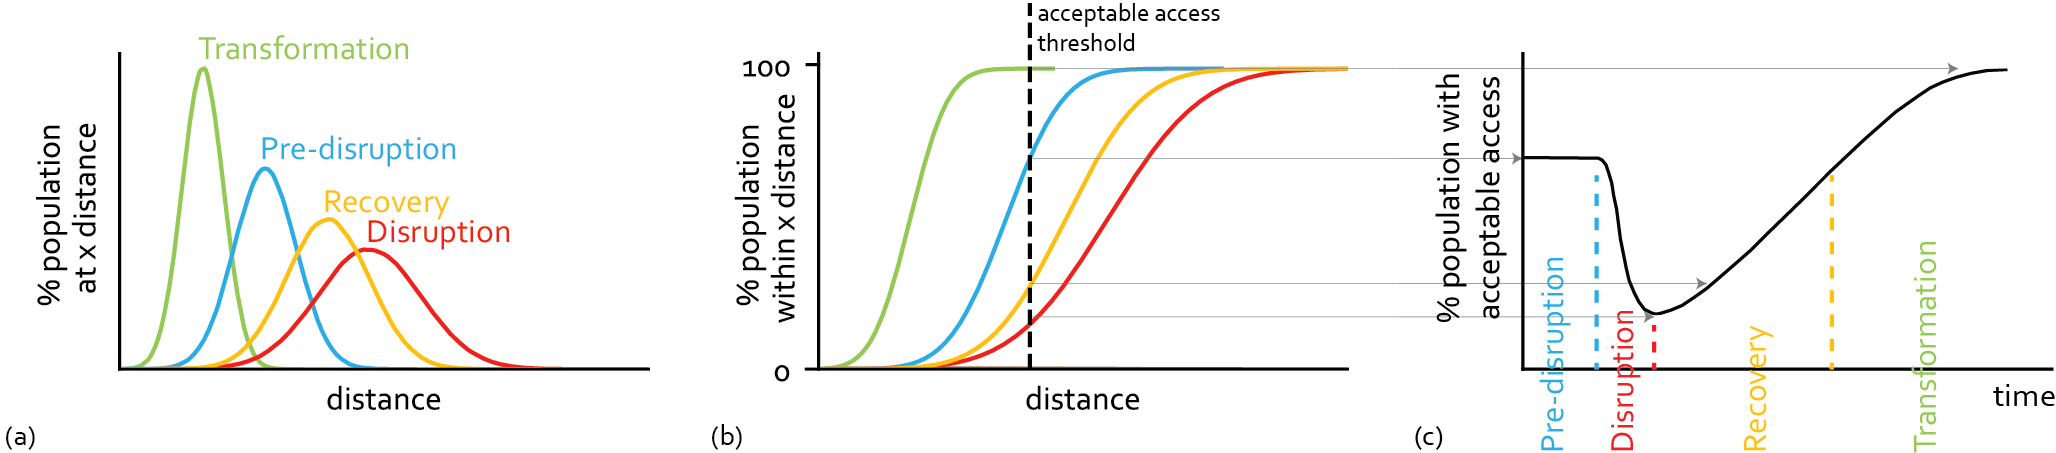
\includegraphics[width=\linewidth]{report/fig/dist_to_resil.png}
    \caption{
    How the distribution of access maps onto the resilience function (aka recovery curve). (a) these are the density functions (idealized histograms) of the distance of residents to their nearest service.
    Each distribution curve represents a different phase of the hazard cycle. 
    (b) these cumulative distribution functions are variants of (a) and show the percentage of the population that live less than the distance on the $x$ axis.
    The threshold of acceptable access is shown here. Where this line intersects with the CDFs we can identify what percentage of the population has acceptable access.
    (c) mapping these values onto their associated time results in this figure that shows acceptable access changing with time, and is a recovery curve.
    }
    \label{figS:cdf_to_res}
\end{figure}

\section*{Extensions}

This approach is suitable for immediate integration into all phases of the hazard cycle. 
Measuring proximity is now practicable and there is real-time information about facility closures. 
Improvements at the implementation level include reliable methods for reporting actual and estimated facility closures and openings. 
These improvements reflect the supply side. 
Improvements to understanding demand include furthering our understanding of the spatial distribution of residents during a disaster.
Integrating cell phone data provides the potential to understand where people have evacuated from, and therefore where emergency supply services should be targeted. 
In the meantime, actionable insight can still be gained from using this approach for emergency response and improving resilience, as we now demonstrate.






%%% Each figure should be on its own page
% \newpage
%  \begin{table}
%      \centering
%      \includegraphics[width=\linewidth]{report/figures/summary_stats.png}
%      \caption{Summary statistics of the variables included in our analysis.}
%      \label{tab:summary_statistics}
%  \end{table}

\begin{figure}
    \centering
    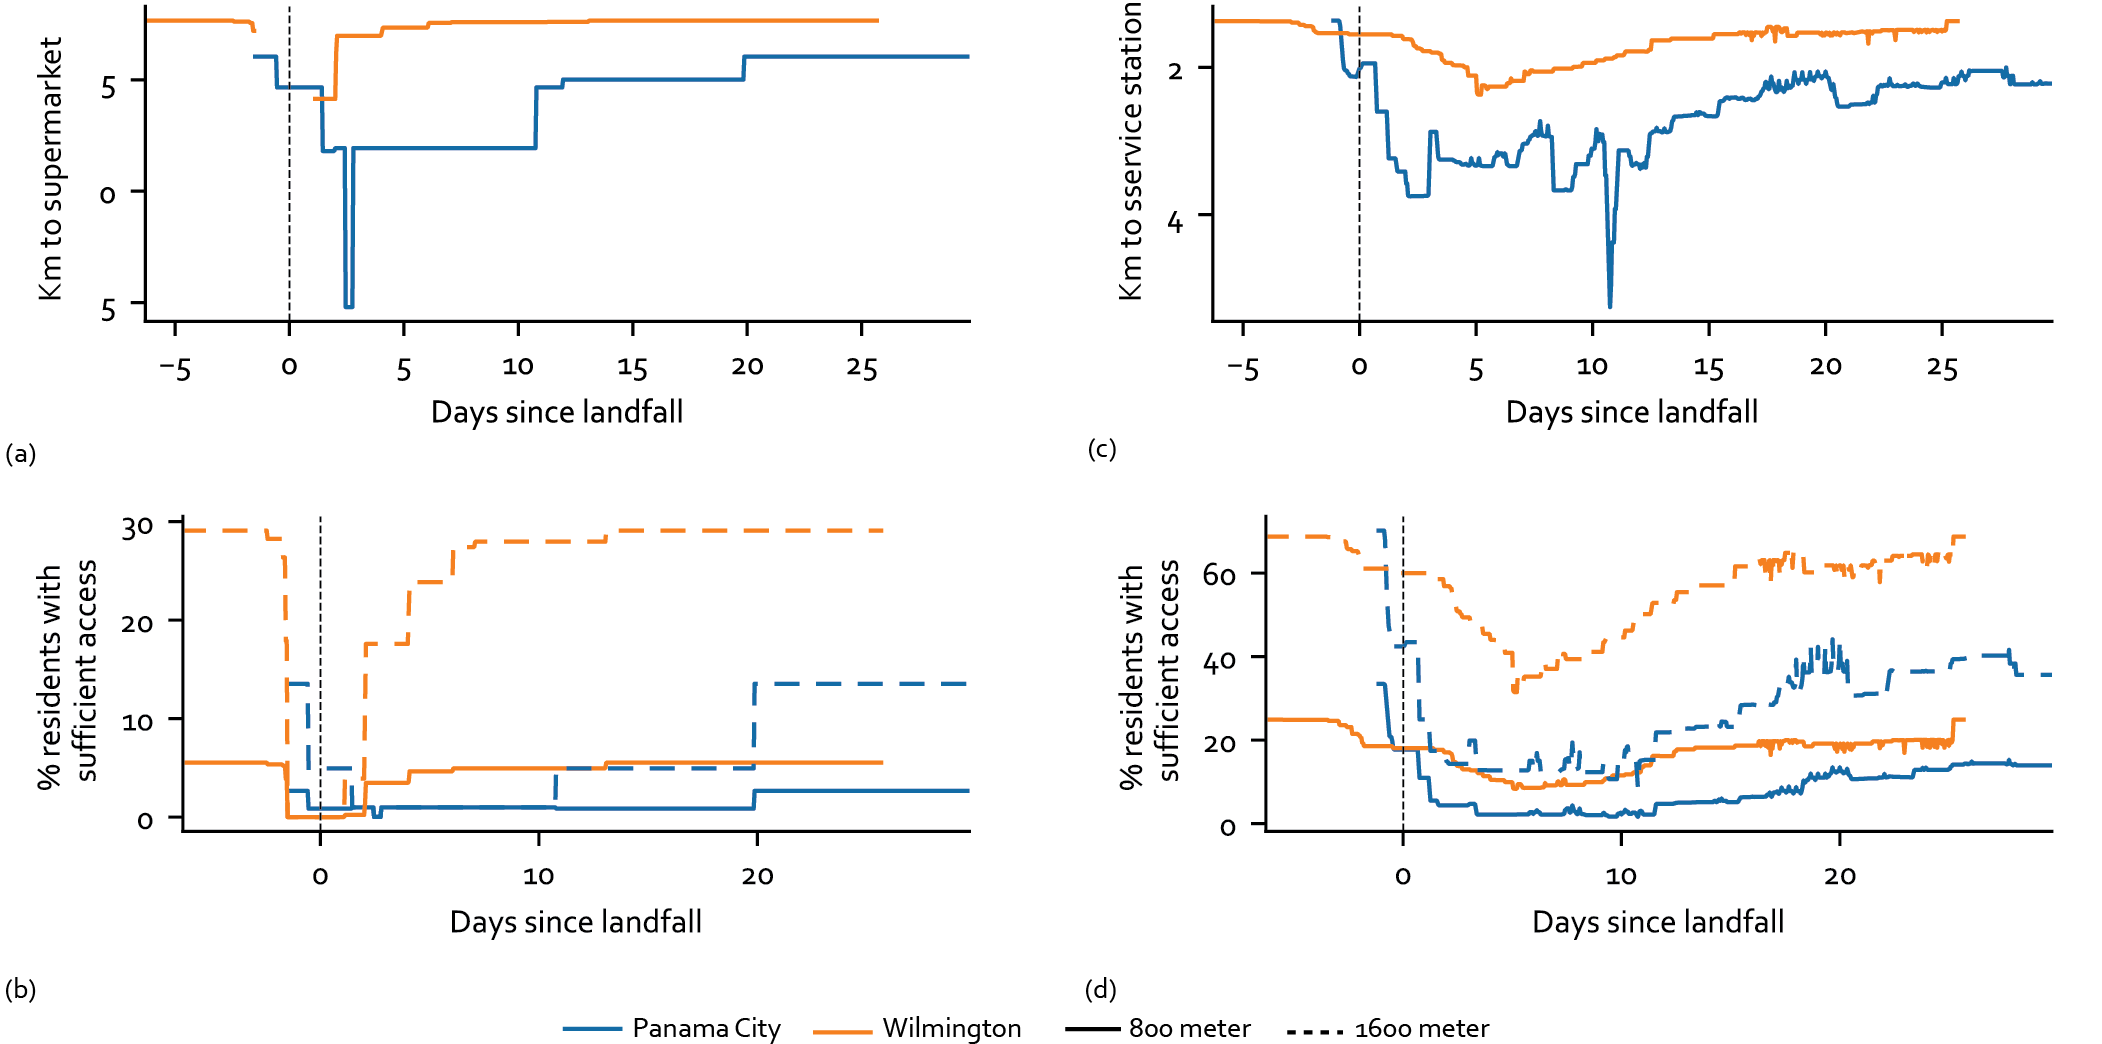
\includegraphics[width=\linewidth]{report/fig/sufficient_access.png}
    \caption{
    Figures (a) and (c) show the distance from nearest service. (b) and (d) show this converted into acceptable access using two threshold distances: 800 and 1600 meters.
    }
    \label{figS:suff_access}
\end{figure}

\begin{figure}
    \centering
    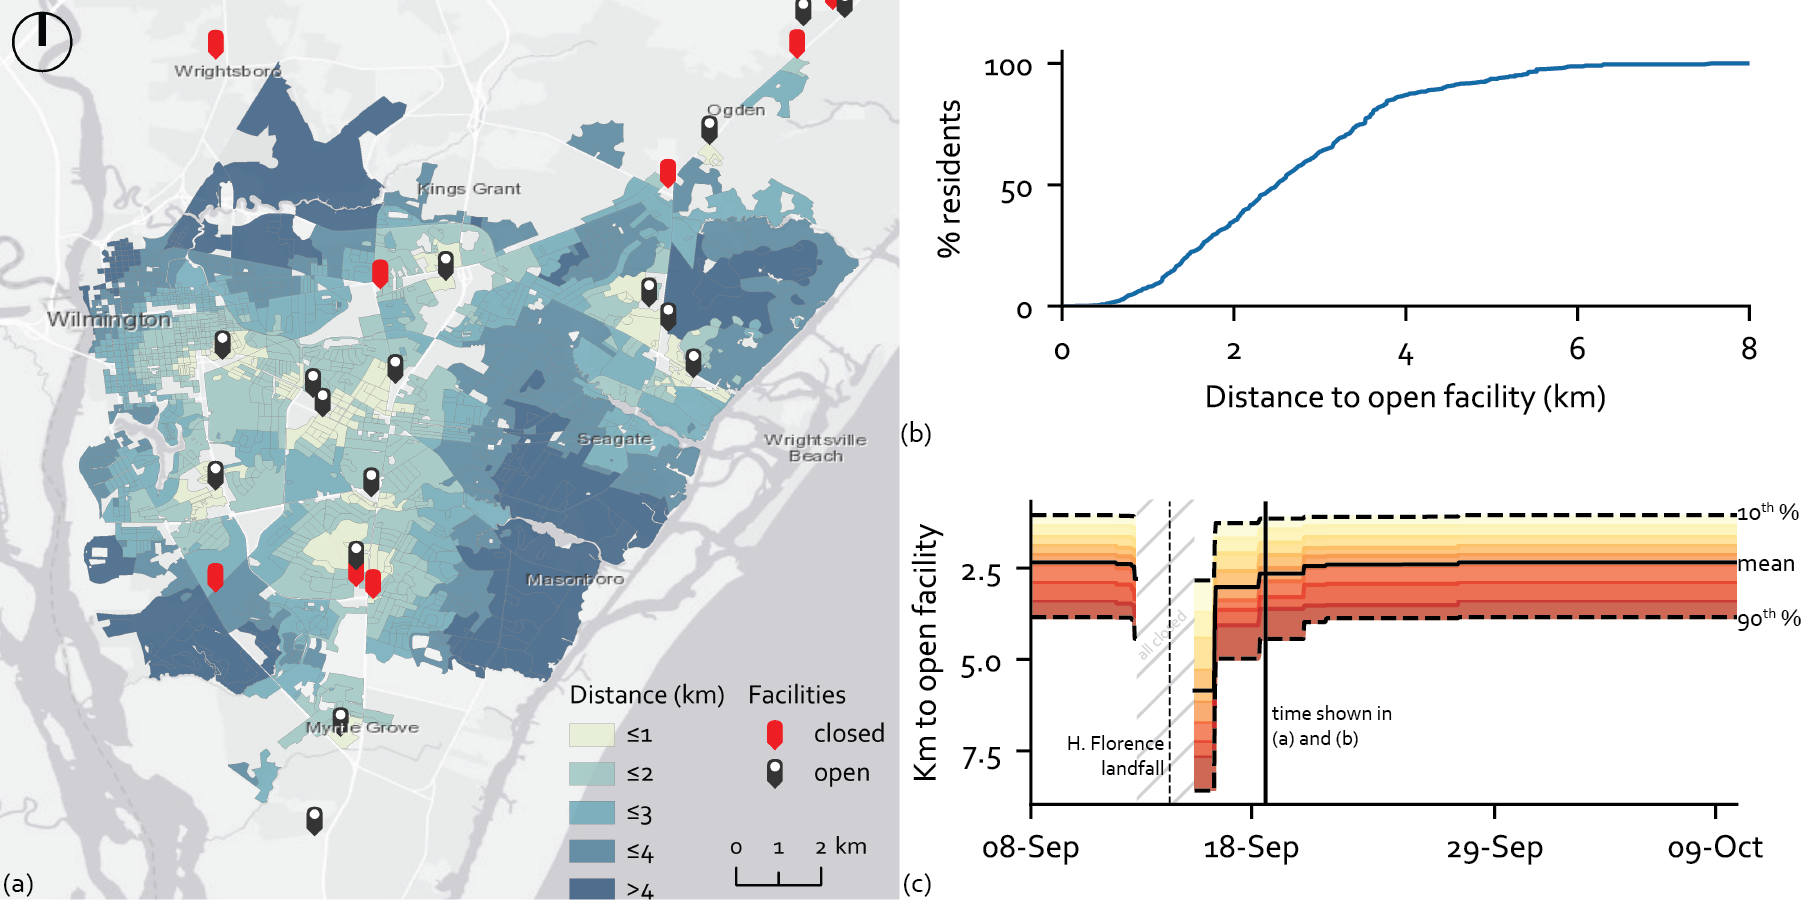
\includegraphics[width=\linewidth]{report/fig/FigS_Wilm_supermarket.png}
    \caption{
    Supermarket access in Wilmington, NC on the 18th of September, 2018. (a) The map of distance to nearest operational service for census blocks with non-zero populations, (b) the cumulative distribution function showing how many residents are closer than $x$ to their nearest operational service, and (c) the resilience curve showing how the distribution in access changes over time.
    }
    \label{figS:nc_grocery}
\end{figure}

\begin{figure}
    \centering
    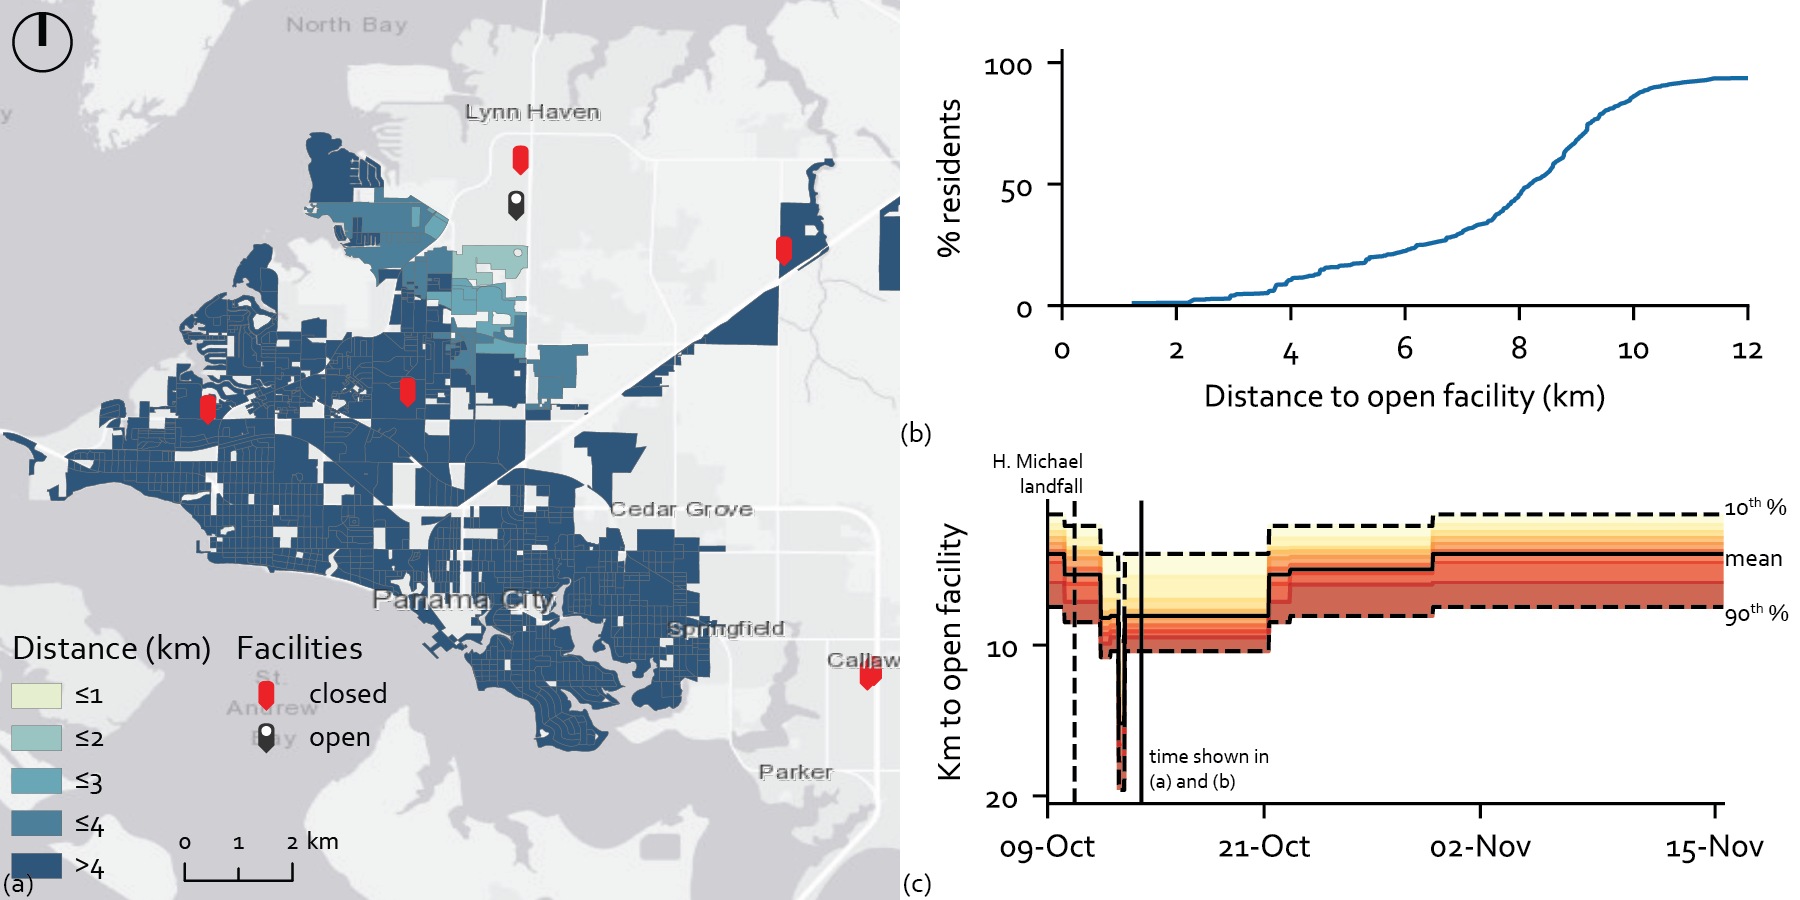
\includegraphics[width=\linewidth]{report/fig/FigS_fl_supermarket.png}
    \caption{
    Supermarket access in Panama City, FL on the 14th of October, 2018. (a) The map of distance to nearest operational service for census blocks with non-zero populations, (b) the cumulative distribution function showing how many residents are closer than $x$ to their nearest operational service, and (c) the resilience curve showing how the distribution in access changes over time.
    }
    \label{figS:fl_grocery}
\end{figure}


\begin{figure}
    \centering
    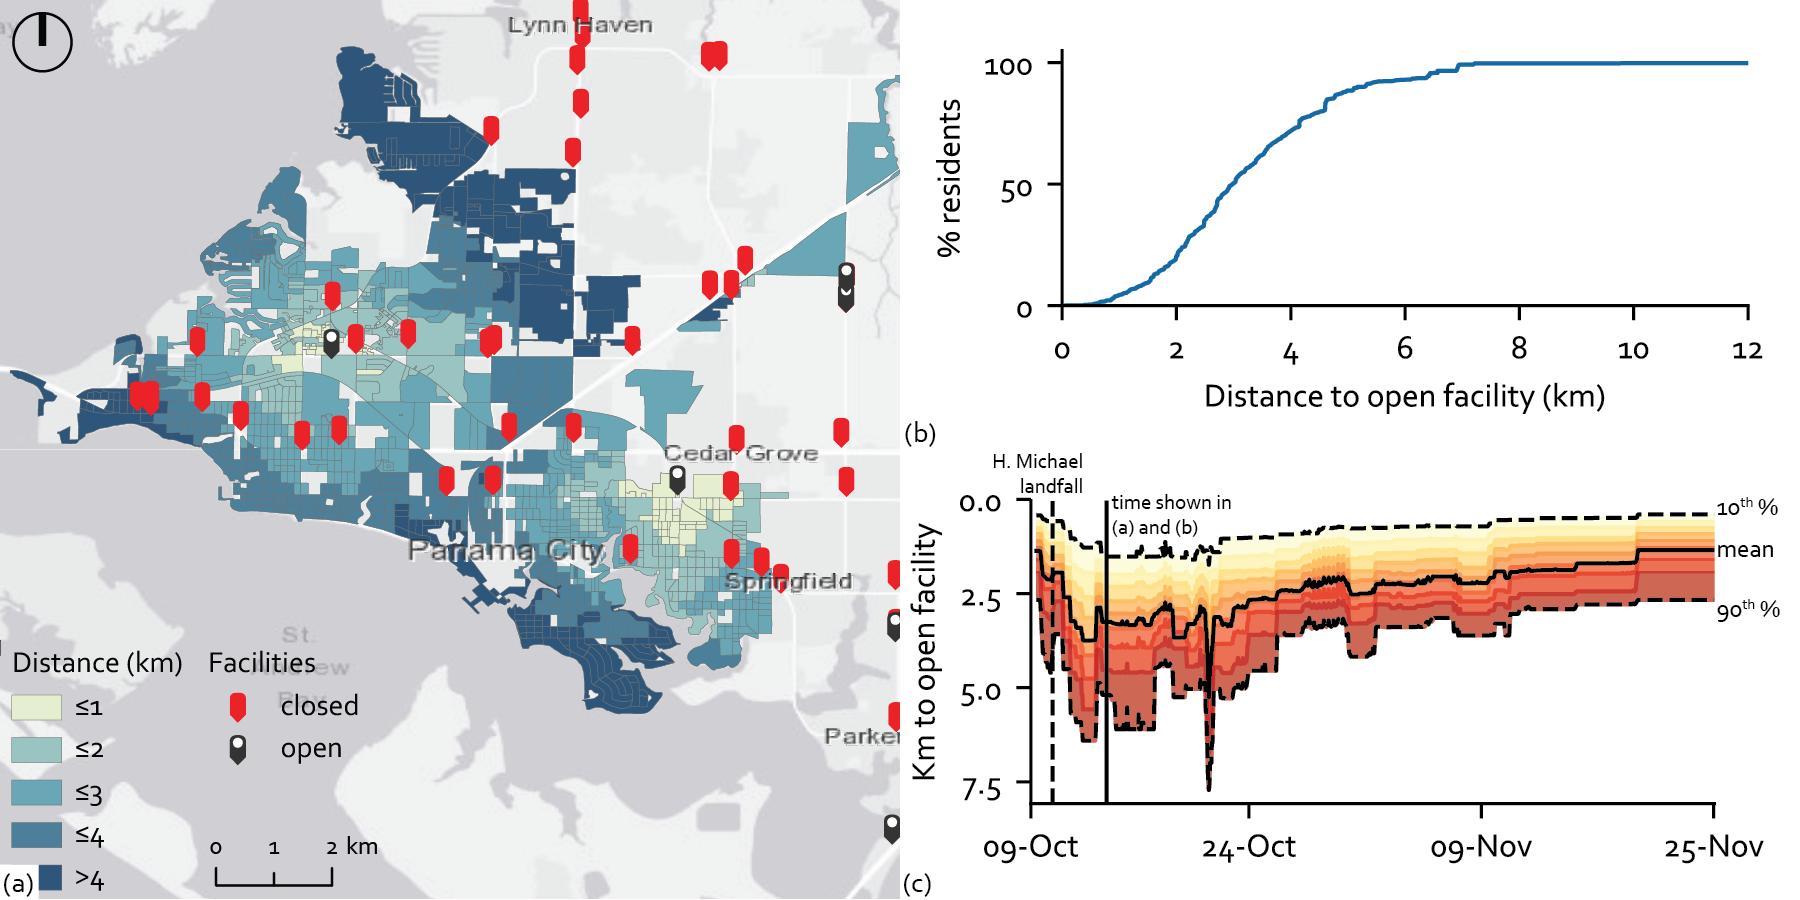
\includegraphics[width=\linewidth]{report/fig/FigS_fl_station.png}
    \caption{
    Service station access in Panama City, FL on the 14th of October, 2018. (a) The map of distance to nearest operational service for census blocks with non-zero populations, (b) the cumulative distribution function showing how many residents are closer than $x$ to their nearest operational service, and (c) the resilience curve showing how the distribution in access changes over time.
    }
    \label{figS:fl_station}
\end{figure}


\end{document}